\documentclass[margin=2pt]{standalone}
\usepackage[table]{xcolor}
\usepackage[utf8]{inputenc}
\usepackage[T1]{fontenc}

\usepackage{tikz}
\usepackage{helvet}
\usepackage{amsmath}

\renewcommand\familydefault\sfdefault

% Use \phantom to hide text for exams
\renewcommand{\phantom}{}

\newcommand{\lOS}{\phantom{Operační}\\\phantom{systém}}
\newcommand{\lTask}{{úloha}}
\newcommand{\lTaskAddressSpace}{\phantom{adresový prostor}\\\phantom{úlohy}}
\newcommand{\lSection}{\phantom{Sekce}}
\newcommand{\lUnallocated}{\phantom{Nepřidělený}\\\phantom{prostor}}

\usetikzlibrary{intersections, shapes.arrows, spath3, shapes.geometric, fit, backgrounds, calc, tikzmark, decorations.pathreplacing, angles, quotes}

\definecolor{themeBlue}{RGB}{1, 103, 143}
\definecolor{themeOrange}{RGB}{221, 109, 16}
\definecolor{themeTeal}{RGB}{18, 54, 69}
\definecolor{themeGrey}{RGB}{120, 121, 124}

\begin{document}
    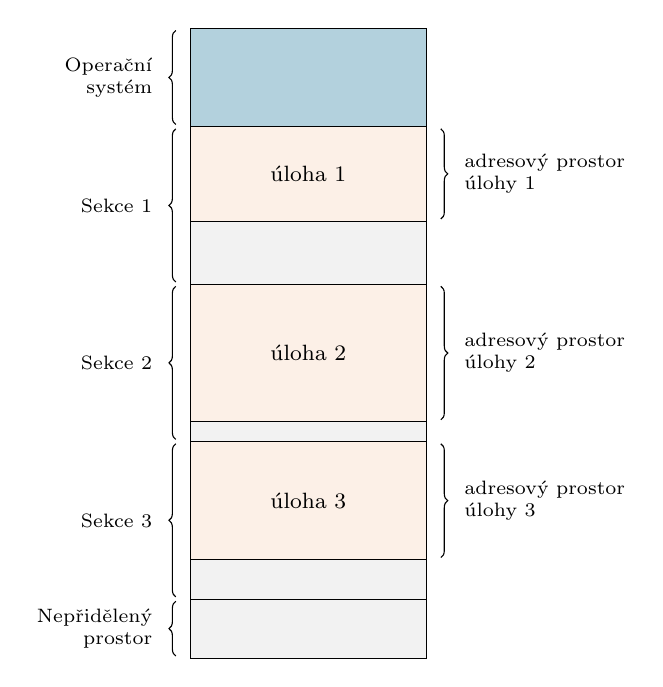
\begin{tikzpicture} [
        width/.style={minimum width=3cm,},
        os/.style={draw, width, anchor=north, minimum height=1.25cm, fill=themeBlue!30},
        task used/.style={draw, width, anchor=north, minimum height=3cm, fill=themeOrange!10, font=\footnotesize},
        task unused/.style={draw, width, anchor=north, minimum height=1cm, fill=themeGrey!10},
        label left/.style={font=\scriptsize, minimum width=1cm, align=right, left=10pt},
        label right/.style={font=\scriptsize, minimum width=1cm, align=left, right=10pt},
        brace mirror/.style={decoration={brace,mirror,raise=5pt}, decorate},
        brace/.style={decoration={brace,raise=5pt}, decorate}
    ]

    \draw node[os] (os) {};
    \coordinate (h0) at (os.south);

    \foreach \size/\scale [count=\i from 1, remember=\i as \h (initialy 0)] in {2/1.2, 2/1.75, 2/1.5} {
        \pgfmathsetmacro{\BlockHeight}{\size}
        \pgfmathsetmacro{\BlockUsed}{\BlockHeight/2*\scale}
        \pgfmathsetmacro{\BlockUnused}{\BlockHeight-\BlockUsed}
        \draw (h\h) node[task used, yshift=\pgflinewidth, minimum height=\BlockUsed cm] (task \i used) { \lTask\space\i };
        \draw (task \i used.south) node[task unused, yshift=\pgflinewidth, minimum height=\BlockUnused cm] (task \i unused) {};
        \coordinate (h\i) at (task \i unused.south);

        \draw[brace mirror]  ($ (task \i used.north west) - (0, 1pt) $) -- node[label left] {\lSection\phantom{\space\i}} ($ (task \i unused.south west) + (0, 1pt) $);

        \draw[brace]  ($ (task \i used.north east) - (0, 1pt) $) -- node[label right] {\lTaskAddressSpace\phantom{\space\i}} ($ (task \i used.south east) + (0, 1pt) $);
    }

    \draw (h3) node[task unused, yshift=\pgflinewidth, minimum height=.75cm] (mem unused) {};
    
    
    \draw[brace mirror]  ($ (os.north west) - (0, 1pt) $) -- node[label left] {\lOS} ($ (os.south west) + (0, 1pt) $);
    \draw[brace mirror]  ($ (mem unused.north west) - (0, 1pt) $) -- node[label left] {\lUnallocated} ($ (mem unused.south west) + (0, 1pt) $);
    
    \end{tikzpicture}
\end{document}
